\documentclass{beamer}
%\usepackage{beamerthemesplit}
\usepackage{CJKutf8}
\usepackage{tikz}
\setbeamertemplate{theorems}[numbered]

\usepackage{ragged2e}
%\justifying\let\raggedright\justifying


\begin{document}
\begin{CJK*}{UTF8}{gbsn}

\newtheorem{Thm}{定理}[section]
\newtheorem{Cor}{推论}[section]
\theoremstyle{definition}
\newtheorem{Def}{定义}[section]
\theoremstyle{example}
\newtheorem*{Ex}{例:}
\newtheorem*{Exercise}{习题}

\date{}
\author{陈建文}

\title{第二章 映射}
\begin{frame}
  \titlepage
\end{frame}  
\section{映射}
\begin{frame}
  \frametitle{1. 映射}
  
  % \begin{Def}
  %   设$X$和$Y$是两个非空集合,$P(x,y)$是定义在$X\times Y$上的一个二元谓词,且满足以下两个条件:
  %   \begin{enumerate}[(1)]
  %   \item 对$X$的每一个元素$x$, 存在$y\in Y$, 使得$P(x,y)$取值为真;
  %   \item 如果$P(x,y_1)$,$P(x, y_2)$同时取值为真,则$y_1 = y_2$。
  %   \end{enumerate}
  %   则$P(x,y)$确定了一个\alert{映射}$f:X\to Y$, 对任何的$x\in X$,$f(x)$定义为$Y$中使得$P(x,y)$为真的唯一的$y$。这里$y$称为$x$在$f$下的\alert{象},而$x$称为$y$的\alert{原象}。
  %   $X$称为$f$的\alert{定义域};集合$\{f(x) | x \in X\}$称为$f$的\alert{值域},记为$Im(f)$。
  % \end{Def}
  \begin{Def}
    设$X$和$Y$为两个集合。一个从$X$到$Y$的\alert{映射}$f$为一个法则,根据$f$,对$X$中的每个元素$x$都有$Y$中唯一确定的元素$y$与之对应。
    从$X$到$Y$的映射$f$常记为$f:X\to Y$。
  \end{Def}\pause

  \begin{Def}
    设$X$和$Y$为两个集合。一个从$X$到$Y$的映射为一个满足以下两个条件的$X\times Y$的子集$f$:
    \begin{enumerate}
    \item 对$X$的每一个元素$x$,存在一个$y\in Y$,使得$(x,y) \in f$;
    \item 若$(x,y)\in f$,$(x,y')\in f$,则$y=y'$。
    \end{enumerate}
    $(x,y)\in f$记为$y=f(x)$。
  \end{Def}\pause

  \begin{Def}\justifying\let\raggedright\justifying
    设$f$为从集合$X$到集合$Y$的映射,$f:X\to Y$, 如果$y = f(x)$,则称$y$为$x$在$f$下的\alert{象},称$x$为$y$的\alert{原象}。$X$称为$f$的\alert{定义域};集合$\{f(x) | x \in X\}$称为$f$的\alert{值域},记为$Im(f)$。
  \end{Def}
\end{frame}
\begin{frame}
  \frametitle{1. 映射}

  \begin{Def}
    设$f:X\to Y$,$A\subseteq X$,当把$f$的定义域限制在$A$上时,就得到了一个
    $\phi: A\to Y$,$\forall x \in A$,$\phi(x) = f(x)$。$\phi$称为$f$在$A$上的
    \alert{限制},并且常用$f|A$来表示$\phi$。反过来,我们也称$f$为$\phi$在$X$上的\alert{扩张}。
  \end{Def}\pause
    \begin{Def}
    设$f:A \to Y$,$A \subseteq X$, 则称$f$为$X$上的一个\alert{部分映射}。
  \end{Def}\pause
  \begin{Def}
    两个映射$f$与$g$称为是\alert{相等}的当且仅当$f$和$g$都为从$X$到$Y$的映射,并且$\forall x \in X$总有$f(x) = g(x)$。
  \end{Def}\pause
  \begin{Def}
    设$f:X\to X$,如果$\forall x \in X, f(x) = x$,则称$f$为$X$上的恒等映射。$X$上的恒等映射常记为$I_X$。
  \end{Def}

\end{frame}

\begin{frame}
  \frametitle{1.映射}
  \begin{Def}\justifying\let\raggedright\justifying
    设$f:X\to Y$,如果$\forall x_1, x_2 \in X$, 只要$x_1 \neq x_2$,  就 有 $f(x_1) \neq f(x_2)$,   则称$f$为从$X$到$Y$的\alert{单射}。
  \end{Def}
  \begin{Def}\justifying\let\raggedright\justifying
    设$f:X\to Y$, 如果$\forall y \in Y$, $\exists x \in X$使得 $f(x) = y$, 则称$f$为从$X$到$Y$的\alert{满射}。
  \end{Def}
  \begin{Def}\justifying\let\raggedright\justifying
    设$f:X\to Y$,如果$f$既是单射又是满射,则称$f$为从$X$到$Y$的\alert{双射},或者称$f$为从$X$到$Y$的\alert{一一对应}。这时也称$X$与$Y$\alert{对等},记为$X\sim Y$。
  \end{Def}

\end{frame}
\begin{frame}
  \frametitle{1.映射}
  \begin{Def}
    从集合$X$到集合$Y$的所有映射之集记为$Y^X$,即$\{f|f:X\to Y\}$。
  \end{Def}
\end{frame}
\section{抽屉原理}
\begin{frame}
  \frametitle{2. 抽屉原理}
  \begin{Thm}[抽屉原理]
    如果把$n+1$个物体放到$n$个盒子里,则必有一个盒子里至少放了两个物体。
  \end{Thm}
  
  %\begin{Ex}
  %  已知$m$个整数$a_1,a_2,\ldots,a_m$,试证:存在两个整数 $k$, $l$, \\ $0\leq k < l \leq m$,使得$a_{k+1}+a_{k+2}+\ldots+a_{l}$能被$m$整除。
  %\end{Ex}
\end{frame}

\begin{frame}
    \frametitle{2. 抽屉原理}
  \begin{Ex}
    从$1,2,\ldots, 2n$中任意选出$n+1$个数,则这$n+1$个数中必有两个数,使得其中之一能除尽另一个。
  \end{Ex}
  \pause
  \begin{proof}[证明]\justifying\let\raggedright\justifying
  每个整数均可写成$2^l\cdot d$的形式,其中$l$为非负整数,$d$为奇数。因此,当把选出的$n+1$个整数都写成这种形式时,便得到了$n+1$个奇数$d_1,d_2,\cdots, d_{n+1}$,并且$1\leq d_i \leq 2n -1$,$i=1,2,\cdots, n+1$。但$1$到$2n$之间仅有$n$个奇数,由抽屉原理可知,必有$i,j$使得$d_i=d_j$,$i\neq j$。于是,$d_i$与$d_j$对应的两个整数$2^{l_i}\cdot {d_i}$与$2^{l_j}\cdot {d_j}$中必有一个可以整除另外一个。
  \end{proof}
\end{frame}

\begin{frame}
    \frametitle{2. 抽屉原理}
  \begin{Ex}
    任何6个人中,或有$3$个人互相认识,或有$3$个人互相不认识。
  \end{Ex}
  
\end{frame}


\begin{frame}
  \frametitle{2. 抽屉原理}
  \begin{Thm}[抽屉原理的强形式]
    设$q_1$,$q_2$,$\ldots$,$q_n$为$n$个正整数。如果把 $q_1 + q_2 + \cdots + q_n$  $- n$ $ + 1$ 个物体放到$n$个盒子中,则或者第一个盒子中至少含有$q_1$个物体,或者第二个盒子中至少含有$q_2$个物体,$\ldots$,
    或者第$n$个盒子中至少含有$q_n$个物体。
  \end{Thm}\pause
  \begin{Cor}
    如果把$n(r-1) + 1$个物体放入$n$个盒子里,则至少有一个盒子里放了不少于$r$个物体。
  \end{Cor}\pause
  \begin{Cor}
    如果$n$个正整数$m_1, m_2, \ldots, m_n$的平均值\[\frac{m_1 + m_2 + \ldots + m_n}{n} > r - 1,\] 则$m_1, m_2, \ldots, m_n$中至少有一个正整数不小于$r$。
  \end{Cor}
\end{frame}

\begin{frame}
    \frametitle{2. 抽屉原理}
  \begin{Ex}
    $n^2+1$个士兵站成一排,则可以使其中的至少$n+1$个士兵向前走一步站成一个按身高从小到大的队列,或站成一个按身高从大到小的队列。
  \end{Ex}
  \begin{proof}[证明]
    \justifying\let\raggedright\justifying
    \pause从左到右依次用$h_1, h_2, \cdots, h_{n^2+1}$表示此队列中各士兵的身高,\pause于是,\pause我们得到了一个$n^2+1$项的数列
    \begin{equation}\label{soldier}
      h_1,h_2,\cdots, h_{n^2+1}
    \end{equation}
    \pause 我们的问题就是要证明此数列中或者有一个长(项数)至少为$n+1$的不减子序列,\pause 或者有一个长至少为$n+1$的不增子序列。

      \end{proof}
\end{frame}
\begin{frame}
  \justifying\let\raggedright\justifying
  \pause假设本题结论不成立,\pause 则数列\eqref{soldier}中每个不减子序列的长度至多为$n$,\pause每个不增子序列的长度也至多为$n$。\pause令$m_i$为以$h_i$为首项的\eqref{soldier}的最长不减子序列的长度,\pause $i=1,2,\cdots, n^2+1$。\pause 于是得到$n^2+1$个数$m_1,m_2,\cdots,m_{n^2+1}$,\pause 其中每个数$m_i$满足$1\leq m_i \leq n$。\pause 现在把这$n^2+1$个数放到$n$个盒子$1,2,\cdots,n$中,\pause 数$m_i$放到第$k$个盒子中当且仅当$m_i=k$,\pause 则必有某个盒子中至少含有$n+1$个数。\pause 由上述方法可知,\pause 在这同一个盒子中的至少$n+1$个数,\pause 它们是相等的。\pause 设这些数为$m_{i_1},m_{i_2},\cdots, m_{i_k}$,\pause $i_1<i_2<\cdots<i_k\leq n^2+1$,$k>n$。\pause 相应的,\pause 我们有\eqref{soldier}的子序列
  \begin{equation}\label{subseq}
  h_{i_1}, h_{i_2}, \cdots, h_{i_k}      
  \end{equation}
 \pause  这是一个不增子序列。\pause 实际上,\pause 如若不然,\pause 例如$h_{i_1} < h_{i_2}$,\pause 则由于以$h_{i_2}$为首项的最长不减子序列的长为$m_{i_2}$,\pause 所以前面加一项$h_{i_1}$,\pause 就得到了一个以$h_{i_1}$为首项长度大于$m_{i_1}$的不减子序列,\pause 这是不可能的。

 \pause  于是,\pause 我们得到了一个长度至少为$n+1$的不增子序列\eqref{subseq},\pause 这又与假设相矛盾。\pause 所以,\pause 本题结论成立。

\end{frame}
\begin{frame}
  \begin{Exercise}
    毕业舞会上,小伙子与姑娘跳舞。已知每个小伙子至少与一个姑娘跳过舞,但未能与所有的姑娘跳过舞。同样的,每个姑娘也至少与一个小伙子跳过舞,但也未能与所有的小伙子跳过舞。证明:在所有参加舞会的小伙子与姑娘中,必可找到两个小伙子与两个姑娘,这两个小伙子中的每一个只与这两个姑娘中的一个跳过舞,而这两个姑娘中的每一个也只与这两个小伙子中的一个跳过舞。
  \end{Exercise}\pause
  \begin{proof}[证法一]
    \pause设小伙子的集合为$B=\{b_1,b_2,\cdots,b_m\}$,\pause姑娘的集合为$G=\{g_1,g_2,\cdots,g_n\}$, \pause $G_{b_i}$为与小伙子$b_i$跳过舞的姑娘的集合,\pause 则由假设$G_{b_i}\neq G$,\pause $i=1,2,\cdots,m$。\pause 如果存在$i, j$,\pause $i \neq j$,\pause 使得$G_{b_i}\nsubseteq G_{b_j}$且$G_{b_j}\nsubseteq G_{b_i}$,\pause则问题得证。\pause否则,\pause对任意的$i$,$j$,\pause或者$G_{b_i}\subseteq G_{b_j}$,\pause或者$G_{b_j}\subseteq G_{b_i}$,\pause于是有\[G_{b_{i_1}}\subseteq G_{b_{i_2}}\subseteq \cdots \subseteq G_{b_{i_m}}\]\pause但由假设,\pause $\bigcup_{i=1}^mG_{b_i} = G$,\pause 即$G_{b_{i_m}}=G$,\pause 所以$b_{i_m}$与所有的姑娘都跳过舞,\pause矛盾。
  \end{proof}
\end{frame}
\begin{frame}
  \begin{Exercise}
    毕业舞会上,小伙子与姑娘跳舞。已知每个小伙子至少与一个姑娘跳过舞,但未能与所有的姑娘跳过舞。同样的,每个姑娘也至少与一个小伙子跳过舞,但也未能与所有的小伙子跳过舞。证明:在所有参加舞会的小伙子与姑娘中,必可找到两个小伙子与两个姑娘,这两个小伙子中的每一个只与这两个姑娘中的一个跳过舞,而这两个姑娘中的每一个也只与这两个小伙子中的一个跳过舞。
  \end{Exercise}\pause
  \begin{proof}[证法二]\pause设$b_1$为与姑娘跳舞最多的小伙子。\pause由$b_1$未能与所有的姑娘跳过舞知,\pause存在一个姑娘$g_2$,\pause $b_1$未能与$g_2$跳过舞。\pause 由每个姑娘至少与一个小伙子跳过舞知,\pause 存在一个小伙子$b_2$与$g_2$跳过舞。\pause 在与小伙子$b_1$跳过舞的姑娘中,\pause 必存在一个姑娘$g_1$未能与小伙子$b_2$跳过舞,\pause 否则与$b_1$为与姑娘跳舞最多的小伙子矛盾。\pause于是,\pause $b_1$与$g_1$跳过舞,\pause但未与$g_2$跳过舞;\pause $b_2$与$g_2$跳过舞,\pause但未与$g_1$跳过舞,\pause结论得证。  
  \end{proof}
  
\end{frame}
\begin{frame}
  \begin{Exercise}\justifying\let\raggedright\justifying
          设$X$为一个非空集合,$A_n\subseteq X$, $A_{n+1}\subseteq A_n$,$n=1,2,3,\cdots$。试证对任意的自然数$n$,
      \[A_n=\bigcup_{m=n}^{\infty}(A_m\cap A_{m+1}^c)\cup \bigcap_{m=n}^{\infty}A_m\]
    \end{Exercise}\pause\centering    
      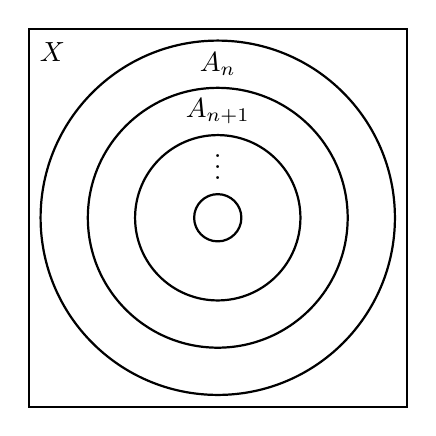
\begin{tikzpicture}[thick, scale=0.3]
    \draw (-8, -8) rectangle (8, 8);
    \draw (0,0) circle [radius=7.5cm];
    \draw (0,0) circle [radius=5.5cm];
    \draw (0,0) circle [radius=3.5cm];
    \draw (0,0) circle [radius=1cm];
    \draw (0,6.5) node {$A_n$};
    \draw (0,4.5) node {$A_{n+1}$};
    \draw (0,2.5) node {$\vdots$};
    \draw (-7,7) node {$X$};
  \end{tikzpicture}
  \end{frame}
  
  \begin{frame}
  \begin{Exercise}\justifying\let\raggedright\justifying
          设$X$为一个非空集合,$A_n\subseteq X$, $A_{n+1}\subseteq A_n$,$n=1,2,3,\cdots$。试证对任意的自然数$n$,
      \[A_n=\bigcup_{m=n}^{\infty}(A_m\cap A_{m+1}^c)\cup \bigcap_{m=n}^{\infty}A_m\]
    \end{Exercise}\pause
  \begin{proof}[证明]\justifying\let\raggedright\justifying
  
        \pause先证$A_n\subseteq \bigcup_{m=n}^{\infty}(A_m\cap A_{m+1}^c)\cup \bigcap_{m=n}^{\infty}A_m$:
      
      \pause对任意的$x\in A_n$,\pause如果$x\in \bigcap_{m=n}^{\infty}A_m$,则$x\subseteq  \bigcup_{m=n}^{\infty}(A_m\cap A_{m+1}^c)\cup \bigcap_{m=n}^{\infty}A_m$;
      \pause如果$x\notin \bigcap_{m=n}^{\infty}A_m$,\pause则存在$i$,$i\geq n$且$x\notin A_i$,\pause取最小的$j$,使得$j\geq n$且$x\notin A_j$,\pause由$x\in A_n$知$j \neq n$,\pause于是$x\in A_{j-1}$但$x\notin A_j$,这里$j>n$,\pause从而$x\in \bigcup_{m=n}^{\infty}(A_m\cap A_{m+1}^c)$,\pause此时亦有$x\subseteq  \bigcup_{m=n}^{\infty}(A_m\cap A_{m+1}^c)\cup \bigcap_{m=n}^{\infty}A_m$。
      
      \pause再证$\bigcup_{m=n}^{\infty}(A_m\cap A_{m+1}^c)\cup \bigcap_{m=n}^{\infty}A_m \subseteq A_n$:
  
      \pause对任意的$x\subseteq  \bigcup_{m=n}^{\infty}(A_m\cap A_{m+1}^c)\cup \bigcap_{m=n}^{\infty}A_m$,\pause如果$x\in \bigcup_{m=n}^{\infty}(A_m\cap A_{m+1}^c)$,\pause则存在$i$,$i\geq n$,$x\in A_i\cap A_{i+1}^c$,\pause由已知条件易知$A_i\subseteq A_n$,\pause从而$x\in A_n$;\pause如果$x\in \bigcap_{m=n}^{\infty}A_m$,\pause则显然$x\in A_n$。
  \end{proof}
  \end{frame}
\begin{frame}
  \begin{Ex}
    设$a_1, a_2, \cdots, a_n$为$n$个实数且$a_1<a_2<\cdots <a_n$。$\varphi$为从$A=\{a_1,a_2,\cdots,a_n\}$到$A$的一一对应。试证:如果$a_1+\varphi(a_1)<a_2+\varphi(a_2)<\cdots < a_n+\varphi(a_n)$,则$\varphi = I_A$。
  \end{Ex}
  \pause
  \begin{proof}[证明]
    \pause设$\varphi(a_1)\neq a_1$,\pause则由$\varphi$为双射知存在$j$,\pause $j>1$,\pause $\varphi(a_j)=a_1$。\pause于是,\pause 对任意的正整数$i<j$,\pause $a_i+\varphi(a_i)<a_j+\varphi(a_j)=a_j+a_1$,\pause 由$a_i\geq a_1$知$\varphi(a_i)< a_j$,\pause 从而$\varphi(a_i)=a_k,k<j$。\pause 于是,\pause 对任意的$i$,\pause $i<j$,\pause $\varphi(a_i)\in \{a_2,\ldots,a_{j-1}\}$,\pause 由鸽笼原理,\pause 必存在$i_1<i_2<j$,\pause $\varphi(i_1)=\varphi(i_2)$,\pause 这与$\varphi$为双射矛盾。\pause 类似可证,\pause $\varphi(a_2)=a_2,\ldots,\varphi(a_n)=a_n$,\pause 即$\varphi = I_A$。
  \end{proof}  
\end{frame}  
\begin{frame}
  \frametitle{2. 抽屉原理}
  \begin{Exercise}
    在一个半径为$16$的圆内任意放入$650$个点。给你一个形似垫圈的圆环,此圆环的外半径为$3$,内半径为$2$。现在要求你用这个垫圈盖住这$650$个点中的至少$10$个点,这可能吗?证明你的结论。
  \end{Exercise}
  \pause
  \begin{proof}[答]
    \pause 用这个垫圈可以盖住$650$个点中的至少$10$个点。\pause以圆内的650个点中的每个点为圆心放一个圆环,\pause则所有圆环的面积之和为$S_1 = 650 * \pi * (3^2 - 2^2) = 3250\pi$。\pause所有圆环所覆盖的区域被包含在一个面积为$\pi * (16 + 3)^2= 361\pi$的圆$C$内。\pause此时必存在$10$个圆环$R_1,R_2,\ldots, R_{10}$有公共的重叠区域,\pause否则所有圆环的面积之和$S_1$将小于圆$C$之面积的$9$倍,\pause即$3250\pi < 9 * 361\pi = 3249\pi$,\pause矛盾。\pause任取圆环$R_1,R_2,\ldots, R_{10}$的公共重叠区域中的一点,\pause在该点上放一个圆环,\pause将覆盖住$R_1,R_2,\ldots,R_{10}$的圆心,\pause这$10$个圆心都是圆内$650$个点中的点,\pause结论得证。 
  \end{proof}
\end{frame}
\section{映射的一般性质}
\begin{frame}
  \frametitle{3. 映射的一般性质}
  \begin{Def}
    设$f:X\to Y$,$A \subseteq X$,$A$在$f$下的\alert{象}定义为\[f(A)=\{f(x)|x\in A\}\]
  \end{Def}\pause
  \begin{Ex}
    设$f:\{-1,0,1\}\to \{0,1,2\}$,$f(x)=x^2$,$f(\{-1,0\})$=?
  \end{Ex}
\end{frame}
\begin{frame}
  \frametitle{3. 映射的一般性质}
  \begin{Def}
    设$f:X\to Y$,$B \subseteq Y$,$B$在$f$下的\alert{原象}定义为\[f^{-1}(B)=\{x\in X|f(x)\in B\}\]
  \end{Def}\pause
  \begin{Ex}
    设$f:\{-1,0,1\}\to \{0,1,2\}$,$f(x)=x^2$,则$f^{-1}(\{1,2\})$=?
  \end{Ex}
\end{frame}

\begin{frame}
  \frametitle{3. 映射的一般性质}
  \begin{Thm}
    设$f:X\to Y$,$C \subseteq Y$,$D \subseteq Y$, 则
    \begin{enumerate}[(1)]
    \item $f^{-1}(C \cup D) = f^{-1}(C) \cup f^{-1}(D)$
    \item $f^{-1}(C \cap D) = f^{-1}(C) \cap f^{-1}(D)$
    \item $f^{-1}(C \setminus D)=f^{-1}(C) \setminus f^{-1}(D)$
    \item $f^{-1}(C^c) = (f^{-1}(C))^c$
    \item $f^{-1}(C \bigtriangleup D) = f^{-1}(C) \bigtriangleup f^{-1}(D)$
    \end{enumerate}
  \end{Thm}
    \begin{Thm}
    设$f:X\to Y$,$A \subseteq X$,$B \subseteq X$, 则
    \begin{enumerate}[(1)]
    \item $f(A \cup B) = f(A) \cup f(B)$
    \item $f(A \cap B) \subseteq f(A) \cap f(B)$
    \item $f(A \setminus B) \supseteq f(A) \setminus f(B)$
    \item $f(A \bigtriangleup B) \supseteq f(A) \bigtriangleup f(B)$
    \end{enumerate}
  \end{Thm}

\end{frame}

\section{映射的合成}
\begin{frame}
  \frametitle{4. 映射的合成}
  \begin{Def}
    设$f:X\to Y$,$g:Y\to Z$为映射,映射$f$与$g$的\alert{合成} $g\circ f:X\to Z$定义为\[(g\circ f)(x) = g(f(x))\]
  \end{Def}
  \pause
\begin{Thm}
  设$f:X \to Y$,$g:Y\to Z$,$h:Z\to W$ 为映射,则 \[ (h \circ g) \circ f = h \circ (g \circ f) \]
\end{Thm}

\end{frame}

\section{逆映射}
\begin{frame}
  \frametitle{5. 逆映射}
  \begin{Def}
     设$f:X\to Y$为双射,$f$的\alert{逆映射}$f^{-1}:Y\to X$定义为:对任意的$y\in Y$,存在唯一的$x$使得$f(x)=y$,则$f^{-1}(y)=x$。
   \end{Def}
   \pause
     \begin{block}{定义5.1'}
     设$f:X\to Y$为一个双射, 则$g:Y\to X, g=\{(y,x)|(x,y)\in f\}$称为$f$的逆映射,记为$g=f^{-1}$。
   \end{block}
        \begin{block}{定义5.1''}
     设$f:X\to Y$为一个映射。如果存在一个映射$g:Y\to X$使得\[f\circ g = I_{Y} \text{且} g\circ f = I_{X},\]则称映射$f$为可逆的,而$g$称为$f$的\alert{逆映射}。
   \end{block}

   \begin{Thm}
     定义5.1'与定义5.1''是等价的。
   \end{Thm}
\end{frame}
\begin{frame}
  \frametitle{5. 逆映射}
  \begin{Thm}
    设$f:X\to Y$为可逆映射,则$(f^{-1})^{-1}=f$。
  \end{Thm}
  \pause
  \begin{Thm}
    设$f:X\to Y$,$g:Y\to Z$都为可逆映射,则$g\circ f$也为可逆映射并且$(g\circ f)^{-1} = f^{-1}\circ g^{-1}$。
  \end{Thm}
\end{frame}
\begin{frame}
  \frametitle{5. 逆映射}
  \begin{Def}\justifying\let\raggedright\justifying
    设$f:X\to Y$为一个映射,如果存在一个映射 $g:Y\to X$ 使 得 $g\circ f = I_X$,
    则称$f$为\alert{左可逆}的,$g$称为$f$的\alert{左逆映射};如果存在一个映射
    $h:Y\to X$ 使 得 $f\circ h=I_Y$,则称$f$为\alert{右可逆}的,$h$称为$f$的\alert{右逆映射}。
  \end{Def}\pause
  \begin{Thm}
    设$f:X\to Y$为一个映射,则
    \begin{enumerate}
    \item $f$左可逆当且仅当$f$为单射;
    \item $f$右可逆当且仅当$f$为满射。
    \end{enumerate}
  \end{Thm}
\end{frame}
\section{置换}
\begin{frame}
  \frametitle{6. 置换}
  \begin{Def}
    有穷集合$S$到自身的一一对应称为$S$上的一个\alert{置换}。如果$|S| = n$, 则$S$上的置换就说成是\alert{$n$次置换}。
  \end{Def}
\justifying\let\raggedright\justifying
设$S=\{1,2,\ldots,n\}$,$\sigma:S\to S$为$S$上的一个置换,$\sigma(1) = k_1$, $\sigma(2) = k_2$,$\ldots$,$\sigma(n) = k_n$,我们用如下的一个表来表示置换$\sigma$:
\[\sigma=\begin{pmatrix}1&2&\ldots&n\\k_1&k_2&\ldots&k_n\end{pmatrix}\]
\small{\begin{Ex}
  设$S=\{1,2,3,4\}$,$\sigma(1) = 3$, $\sigma(2) = 2$, $\sigma(3) = 4$, $\sigma(4) = 1$,则$\sigma$可以表示为
  \[\sigma=\begin{pmatrix}1&2&3&4\\3&2&4&1\end{pmatrix}\]
  这里,列的次序无关紧要,例如,$\sigma$还可以表示为
  \[\sigma=\begin{pmatrix}2&1&3&4\\2&3&4&1\end{pmatrix}\]
\end{Ex}}
\end{frame}
\begin{frame}
  \frametitle{6. 置换} 
  \begin{Def}
    设$\alpha$与$\beta$为集合$S$上的两个置换,则$\alpha$与$\beta$为两个从$S$到$S$的双射,讨论置换时,我们用$\alpha\beta$表示$\alpha$与$\beta$的合成$\beta \circ \alpha$。
    注意这里$\alpha$与$\beta$的次序,从运算的角度看有一定的便利性,但也有的教材中采用相反的顺序。按照我们的写法,讨论置换时,如果$i \in S$,则用$(i)\alpha$表示$i$在$\alpha$下的像,简记为$i\alpha$。
  \end{Def}
  % \begin{Ex}
  %   设$S=\{1,2,3\}$,$\alpha$和$\beta$为$S$上的两个置换,
  %   \[\alpha=\begin{pmatrix}1&2&3\\1&3&2\end{pmatrix},\beta=\begin{pmatrix}1&2&3\\2&3&1\end{pmatrix}\],
  %   则
  %   \[\alpha\beta=\begin{pmatrix}1&2&3\\1&3&2\end{pmatrix}\begin{pmatrix}1&2&3\\2&3&1\end{pmatrix}=\begin{pmatrix}1&2&3\\2&1&3\end{pmatrix}\],    
  % \end{Ex}
 \end{frame}

 \begin{frame}
  \frametitle{6. 置换} 
  若$\alpha$与$\beta$为两个$n$次置换,当把$\beta$的表示式中的上一行按$\alpha$的下一行的顺序写出时,则$\alpha \beta$的下一行就是$\beta$的新表示式中的下一行。
  % \begin{Ex}
  %   设$S=\{1,2,3\}$,$\alpha$和$\beta$为$S$上的两个置换,
  %   \[\alpha=\begin{pmatrix}1&2&3\\1&3&2\end{pmatrix},\beta=\begin{pmatrix}1&2&3\\2&3&1\end{pmatrix}\],
  %   则
  %   \[\alpha\beta=\begin{pmatrix}1&2&3\\1&3&2\end{pmatrix}\begin{pmatrix}1&2&3\\2&3&1\end{pmatrix}=\begin{pmatrix}1&2&3\\1&3&2\end{pmatrix}\begin{pmatrix}1&3&2\\2&1&3\end{pmatrix}=\begin{pmatrix}1&2&3\\2&1&3\end{pmatrix}\],    
  % \end{Ex}   
 \end{frame}
 \begin{frame}
   \frametitle{6. 置换}
   \begin{Def}\justifying\let\raggedright\justifying
     设$\sigma$为$S$上的一个$n$次置换,若$i_1\sigma=i_2$,$i_2\sigma = i_3$, $\cdots$, $i_{k-1}\sigma = i_k$, $i_k\sigma = i_1$,而$\forall i \in S\setminus \{i_1, i_2, \ldots, i_k\}$, $i\sigma = i$,
     则称$\sigma$为一个\alert{$k$循环置换},记为$(i_1i_2\cdots i_k)$。 $2-$循环置换称为\alert{对换}。
   \end{Def}
   % \begin{Ex}
   % 设$S=\{1,2,3,4,5\}$,则$(1 2 3)=\begin{pmatrix}1&2&3&4&5\\2&3&1&4&5\end{pmatrix}$,$(2 3)=\begin{pmatrix}1&2&3&4&5\\1&3&2&4&5\end{pmatrix}$     
   % \end{Ex}
 \end{frame}

 \begin{frame}
   \frametitle{6. 置换}
   \begin{Thm}
    每个置换都能被分解成若干个没有共同数字的循环置换的乘积。如果不计这些循环置换的顺序以及略去的$1-$循环置换,这个分解是唯一的。
   \end{Thm}
 \end{frame}

 \begin{frame}
   \frametitle{6. 置换}
   \begin{Thm}
    当$n\geq 2$时,每个$n$次置换都能被分解成若干个对换的乘积。
   \end{Thm}
 \end{frame}

 \begin{frame}
   \frametitle{6. 置换}
   \begin{Thm}
    如果把置换分解成若干个对换的乘积,则对换个数的奇偶性是不变的。
  \end{Thm}
  \pause
  \begin{Def}
    能被分解为偶数个对换的乘积的置换称为\alert{偶置换};能被分解为奇数个对换的乘积的置换称为\alert{奇置换}。
  \end{Def}
  \pause
  \begin{Thm}
    当$n \geq 2$时, $n$次奇置换的个数与$n$次偶置换的个数相等,都等于$\frac{n!}{2}$。
  \end{Thm}
 \end{frame}

 
\section{代数运算}
\begin{frame}
  \frametitle{7. 代数运算}
  \begin{Def}
    一个集合及其在该集合上定义的若干个代数运算合称为一个\alert{代数系}。
  \end{Def}

  
    设$x, y, z \in \mathbb{R}$,则
   \begin{enumerate}
   \item   $x + y = y + x$
   \item   $(x + y) + z = x + (y + z)$
   \item   $0 + x = x + 0 = x$
   \item   $(-x) + x =x + (-x) = 0$
   \item   $x * y = y * x$
   \item   $(x * y) * z = x * (y *z)$
   \item   $1 * x = x * 1 = x$
   \item   $x^{-1} * x = x * x^{-1} = 1$
   \item   $x* (y + z) = x * y + x * z$
   \item   $(y + z) * x = y * x + z * x$
    \end{enumerate}
 
\end{frame}

\begin{frame}
    \begin{enumerate}
  \item 对任意的$x\in R$,$y\in R$,$x<y$,$x=y$,$y<x$中有且仅有一个成立。 
  \item 对任意的$x\in R$,$y\in R$,$z\in R$,如果$x<y$并且$y<z$,则$x<z$。
  \item 对任意的$x\in R$,$y\in R$,$z\in R$,如果$x<y$,则$x+z<y+z$。
  \item 对任意的$x\in R$,$y\in R$,如果$x>0$,$y>0$,则$xy>0$。
  \end{enumerate}
\end{frame}
\begin{frame}
    另外,实数集还具有如下性质:

  设$A_1$, $A_2$,$\cdots$,$A_i$,$\cdots$为实数集$R$上的闭区间,$A_1\supseteq A_2 \supseteq A_3 \supseteq \cdots \supseteq A_i \supseteq \cdots$,则$\bigcap_{i=1}^{\infty}A_i$非空。
\end{frame}
\section{代数运算}
\begin{frame}
  \frametitle{7. 代数运算}
  \begin{minipage}[t]{0.5\linewidth}
    设$x, y, z \in \mathbb{R}$,则
   \begin{enumerate}
   \item   $x + y = y + x$
   \item   $(x + y) + z = x + (y + z)$
   \item   $0 + x = x + 0 = x$
   \item   $(-x) + x =x + (-x) = 0$
   \item   $x * y = y * x$
   \item   $(x * y) * z = x * (y *z)$
   \item   $1 * x = x * 1 = x$
   \item   $x^{-1} * x = x * x^{-1} = 1$
   \item   $x* (y + z) = x * y + x * z$
   \item   $(y + z) * x = y * x + z * x$
    \end{enumerate}
\end{minipage}\pause
\begin{minipage}[t]{0.5\linewidth}
  \begin{Def}
    设$X$,$Y$,$Z$为任意三个非空集合。一个 从 $X\times Y$到$Z$的映射 $\phi$ 称 为 $X$与$Y$到$Z$的一个\alert{二元(代数)运算}。当$X=Y=Z$时,则称$\phi$为$X$上的\alert{二元(代数)运算}。
  \end{Def}
\end{minipage}
\end{frame}
\begin{frame}
  \frametitle{7. 代数运算}
  \begin{minipage}[t]{0.49\linewidth}
  \begin{block}{}
    设$x, y, z \in \mathbb{R}$,则
   \begin{enumerate}
   \item   $x + y = y + x$
   \item   $(x + y) + z = x + (y + z)$
   \item   $0 + x = x + 0 = x$
   \item   $(-x) + x =x + (-x) = 0$
   \item   $x * y = y * x$
   \item   $(x * y) * z = x * (y *z)$
   \item   $1 * x = x * 1 = x$
   \item   $x^{-1} * x = x * x^{-1} = 1$
   \item   $x* (y + z) = x * y + x * z$
   \item   $(y + z) * x = y * x + z * x$
    \end{enumerate}
  \end{block}\pause
\end{minipage}
\begin{minipage}[t]{0.49\linewidth}
  \begin{Def}
    从集合$X$到$Y$的任一映射称为从$X$到$Y$的\alert{一元(代数)运算}。如果$X=Y$,则从$X$到$X$的映射称为$X$上的\alert{一元(代数)运算}。
  \end{Def}
\end{minipage}
\end{frame}

\begin{frame}
  \frametitle{7. 代数运算}
  \begin{minipage}[t]{0.49\linewidth}
  \begin{block}{}
    设$x, y, z \in \mathbb{R}$,则
   \begin{enumerate}
   \item   $x + y = y + x$
   \item   $(x + y) + z = x + (y + z)$
   \item   $0 + x = x + 0 = x$
   \item   $(-x) + x = x + (-x) = 0$
   \item   $x * y = y * x$
   \item   $(x * y) * z = x * (y *z)$
   \item   $1 * x = x * 1 = x$
   \item   $x^{-1} * x = x * x^{-1} = 1$
   \item   $x* (y + z) = x * y + x * z$
   \item   $(y + z) * x = y * x + z * x$
    \end{enumerate}
  \end{block}\pause
\end{minipage}
\begin{minipage}[t]{0.49\linewidth}
  \begin{Def}
    设$A_1, A_2, \cdots, A_n, D$为非空集合。一个从 $A_1\times A_2\times \cdots \times A_n$到$D$的映射$\phi$称为$A_1, A_2, \cdots, A_n$到$D$的一个\alert{$n$元(代数)运算}。
    如果$A_1=A_2=\cdots=A_n=D=A$,则称$\phi$为$A$上的\alert{$n$元代数运算}。
  \end{Def}
\end{minipage}
\end{frame}

\begin{frame}
  \frametitle{7. 代数运算}
  \begin{minipage}[t]{0.49\linewidth}
  \begin{block}{}
    设$x, y, z \in \mathbb{R}$,则
   \begin{enumerate}
   \item   $x + y = y + x$
   \item   $(x + y) + z = x + (y + z)$
   \item   $0 + x = x + 0 = x$
   \item   $(-x) + x = x + (-x) = 0$
   \item   $x * y = y * x$
   \item   $(x * y) * z = x * (y *z)$
   \item   $1 * x = x * 1 = x$
   \item   $x^{-1} * x = x * x^{-1} = 1$
   \item   $x* (y + z) = x * y + x * z$
   \item   $(y + z) * x = y * x + z * x$
    \end{enumerate}
  \end{block}\pause
\end{minipage}
\begin{minipage}[t]{0.49\linewidth}
  \begin{Def}
    设“$\circ$”为集合$X$上的一个二元代数运算。如果$\forall a, b \in X$,恒有\\$a \circ b = b \circ a$, 则称二元代数运算“$\circ$”满足\alert{交换律}。
  \end{Def}
\end{minipage}
\end{frame}

\begin{frame}
  \frametitle{7. 代数运算}
  \begin{minipage}[t]{0.49\linewidth}
  \begin{block}{}
    设$x, y, z \in \mathbb{R}$,则
   \begin{enumerate}
   \item   $x + y = y + x$
   \item   $(x + y) + z = x + (y + z)$
   \item   $0 + x = x + 0 = x$
   \item   $(-x) + x =  x + (-x) = 0$
   \item   $x * y = y * x$
   \item   $(x * y) * z = x * (y *z)$
   \item   $1 * x = x * 1 = x$
   \item   $x^{-1} * x = x * x^{-1} = 1$
   \item   $x* (y + z) = x * y + x * z$
   \item   $(y + z) * x = y * x + z * x$
    \end{enumerate}
  \end{block}\pause
\end{minipage}
\begin{minipage}[t]{0.49\linewidth}
  \begin{Def}
    设“$\circ$”为集合$X$上的一个二元代数运算。如果$\forall a, b, c \in X$,恒有$(a \circ b) \circ c = a \circ (b \circ c)$, 则称二元代数运算“$\circ$”满足\alert{结合律}。
  \end{Def}
\end{minipage}
\end{frame}

\begin{frame}
  \frametitle{7. 代数运算}
  \begin{minipage}[t]{0.49\linewidth}
  \begin{block}{}
    设$x, y, z \in \mathbb{R}$,则
   \begin{enumerate}
   \item   $x + y = y + x$
   \item   $(x + y) + z = x + (y + z)$
   \item   $0 + x = x + 0 = x$
   \item   $(-x) + x = x + (-x) = 0$
   \item   $x * y = y * x$
   \item   $(x * y) * z = x * (y *z)$
   \item   $1 * x = x * 1 = x$
   \item   $x^{-1} * x = x * x^{-1} = 1$
   \item   $x* (y + z) = x * y + x * z$
   \item   $(y + z) * x = y * x + z * x$
    \end{enumerate}
  \end{block}\pause
\end{minipage}
\begin{minipage}[t]{0.49\linewidth}
  \begin{Def}
    设“$+$”与“$\circ$”为集合$X$上的两个二元代数运算。\\如果$\forall a, b, c \in X$,恒有\[a \circ (b + c) = a \circ b + a \circ c,\] 则称二元代数运算“$\circ$”对“$+$”满足\alert{左分配律}。
    \\如果$\forall a, b, c \in X$,恒有\[(b + c)\circ a = b \circ a + c \circ a,\] 则称二元代数运算“$\circ$”对“$+$”满足\alert{右分配律}。
  \end{Def}
\end{minipage}
\end{frame}

\begin{frame}
  \frametitle{7. 代数运算}
  \begin{minipage}[t]{0.49\linewidth}
  \begin{block}{}
    设$x, y, z \in \mathbb{R}$,则
   \begin{enumerate}
   \item   $x + y = y + x$
   \item   $(x + y) + z = x + (y + z)$
   \item   $0 + x = x + 0 = x$
   \item   $(-x) + x = x + (-x) = 0$
   \item   $x * y = y * x$
   \item   $(x * y) * z = x * (y *z)$
   \item   $1 * x = x * 1 = x$
   \item   $x^{-1} * x = x * x^{-1} = 1$
   \item   $x* (y + z) = x * y + x * z$
   \item   $(y + z) * x = y * x + z * x$
    \end{enumerate}
  \end{block}\pause
\end{minipage}
\begin{minipage}[t]{0.49\linewidth}
  \begin{Def}
    设$(X, \circ)$为一个代数系。如果存在一个元素$e\in X$使得对任意的$x\in X$恒有$e\circ x = x \circ e = x$, 则称$e$为“$\circ$”的\alert{单位元素}。
  \end{Def}
\end{minipage}
\end{frame}

\begin{frame}
  \frametitle{7. 代数运算}
  \begin{minipage}[t]{0.49\linewidth}
  \begin{block}{}
    设$x, y, z \in \mathbb{R}$,则
   \begin{enumerate}
   \item   $x + y = y + x$
   \item   $(x + y) + z = x + (y + z)$
   \item   $0 + x = x + 0 = x$
   \item   $(-x) + x = x + (-x) = 0$
   \item   $x * y = y * x$
   \item   $(x * y) * z = x * (y *z)$
   \item   $1 * x = x * 1 = x$
   \item   $x^{-1} * x = x * x^{-1} = 1$
   \item   $x* (y + z) = x * y + x * z$
   \item   $(y + z) * x = y * x + z * x$
    \end{enumerate}
  \end{block}\pause
\end{minipage}
\begin{minipage}[t]{0.49\linewidth}
  \begin{Def}
    设$(X, \circ)$为一个代数系,“$\circ$”有单位元素$e$,$a\in X$,如果$\exists b\in X$使得\[a\circ b = b \circ a = e,\]  则称$b$为$a$的\alert{逆元素}。
  \end{Def}
\end{minipage}
\end{frame}

\begin{frame}
  \frametitle{7. 代数运算}
  \begin{Def}
    设$(S,+)$与$(T, \oplus)$为两个代数系。如果存在一个一一对应$\phi:S\to T$, 使得$\forall x, y \in S$,有
    \begin{align*}
      \phi(x+y) &= \phi(x) \oplus \phi(y),
    \end{align*}
    则称代数系$(S,+)$与$(T, \oplus)$\alert{同构},并记为$S\cong T$, $\phi$称为这两个代数系之间的一个同构。
  \end{Def}
\end{frame}

\begin{frame}
  \frametitle{7. 代数运算}
  \begin{Def}
    设$(S,+, \circ)$与$(T, \oplus, *)$为两个代数系。如果存在一个一一对应$\phi:S\to T$, 使得$\forall x, y \in S$,有
    \begin{align*}
      \phi(x+y) &= \phi(x) \oplus \phi(y),\\
      \phi(x\circ y)&= \phi(x) * \phi(y),
    \end{align*}
    则称代数系$(S,+,\circ)$与$(T, \oplus, *)$\alert{同构},并记为$S\cong T$, $\phi$称为这两个代数系之间的一个同构。
  \end{Def}
\end{frame}

\begin{frame}
  \frametitle{7. 代数运算}
  \begin{tabular}{cc|c}
    p& q& p $\land$ q\\
    \hline
    T&T&T\\
    T&F&F\\
    F&T&F\\
    F&F&F\\
  \end{tabular}\hspace{1cm}
  \begin{tabular}{cc|c}
    p& q& p $\lor$ q\\
    \hline
    T&T&T\\
    T&F&T\\
    F&T&T\\
    F&F&F\\
  \end{tabular}\hspace{1cm}
  \begin{tabular}{c|c}
    p& $\lnot$ p\\
    \hline
    T&F\\
    F&T\\
  \end{tabular}

  \vspace{1cm}\pause
    \begin{tabular}{cc|c}
    x& y& x $\land$ y\\
    \hline
    1&1&1\\
    1&0&0\\
    0&1&0\\
    0&0&0\\
  \end{tabular}\hspace{1cm}
  \begin{tabular}{cc|c}
    x& y& x $\lor$ y\\
    \hline
    1&1&1\\
    1&0&1\\
    0&1&1\\
    0&0&0\\
  \end{tabular}\hspace{1cm}
  \begin{tabular}{c|c}
    x& $\bar{x}$\\
    \hline
    1&0\\
    0&1\\
  \end{tabular}
  
代数系$(\{T,F\},\land,\lor,\lnot)$与$(\{1,0\},\land, \lor,\bar{ })$是同构的。
\end{frame}

\section{集合的特征函数}
\begin{frame}
  \frametitle{8. 集合的特征函数}
  \begin{Def}
    设$X$为一个集合,$E \subseteq X$。 $E$的\alert{特征函数}$\chi_E:X\to \{0,1\}$定义为
    \begin{equation*}
      \chi_E(x)=
      \begin{cases}
        1 & \text{如果} x \in E,\\
        0 & \text{如果} x \notin E.
      \end{cases}
    \end{equation*}
  \end{Def}
\end{frame}
\begin{frame}
  \frametitle{8. 集合的特征函数}
  \begin{Def}
    令$Ch(X) = \{\chi |\chi:X \to \{0,1\}\}$。
    $\forall \chi, \chi' \in Ch(X)$及$x \in X$,
    \begin{align}
      (\chi \lor \chi')(x) &= \chi(x) \lor \chi'(x)\nonumber\\
      (\chi \land \chi')(x) &= \chi(x) \land \chi'(x)\nonumber\\
      \bar{\chi}(x) &=   \overline{\chi(x)}
    \end{align}
  \end{Def}
  \begin{Thm}
    设$X$为一个集合,则代数系$(2^X, \cup, \cap, ^c)$与$(Ch(X), \lor, \land, \bar{} \ )$同构。
  \end{Thm}
\end{frame}

\begin{frame}
  \begin{align*}
    X=\{&1,2,3\}\\
    2^X=\{&\\
        \phi,&\hspace{1.5cm}\chi_1:X\to \{0,1\}\hspace{0.5cm} \chi_1(1)=0,\chi_1(2)=0,\chi_1(3)=0\\
    \{1\},&\hspace{1.5cm}\chi_2:X\to \{0,1\}\hspace{0.5cm} \chi_2(1)=1,\chi_2(2)=0,\chi_2(3)=0\\
        \{2\},&\hspace{1.5cm}\chi_3:X\to \{0,1\}\hspace{0.5cm} \chi_3(1)=0,\chi_3(2)=1,\chi_3(3)=0\\
    \{3\},&\hspace{1.5cm}\chi_4:X\to \{0,1\}\hspace{0.5cm} \chi_4(1)=0,\chi_4(2)=0,\chi_4(3)=1\\
    \{1,2\},&\hspace{1.5cm}\chi_5:X\to \{0,1\}\hspace{0.5cm} \chi_5(1)=1,\chi_5(2)=1,\chi_5(3)=0\\
    \{2,3\},&\hspace{1.5cm}\chi_6:X\to \{0,1\}\hspace{0.5cm} \chi_6(1)=0,\chi_6(2)=1,\chi_6(3)=1\\
    \{1,3\},&\hspace{1.5cm}\chi_7:X\to \{0,1\}\hspace{0.5cm} \chi_7(1)=1,\chi_7(2)=0,\chi_7(3)=1\\
    \{1,2,3\}&\hspace{1.5cm}\chi_8:X\to \{0,1\}\hspace{0.5cm} \chi_8(1)=1,\chi_8(2)=1,\chi_8(3)=1\\
    \}\\
  \end{align*}
\end{frame}
\begin{frame}
  \frametitle{习题}
    \begin{Exercise}
  设$X=\{a,b,c\}, Y=\{0,1\}, Z=\{2,3\}$。$f:X \to Y, f(a) = f(b) = 0, f(c) = 1$;
  $g:Y\to Z, g(0) = 2, g(1) = 3$。试求$g\circ f$。
  \end{Exercise}
  \begin{Exercise}
    设$f:X \to Y$,$C \subseteq Y$,$D \subseteq Y$,证明

    $f^{-1}(C \setminus D) = f^{-1}(C) \setminus f^{-1}(D)$
  \end{Exercise}
    \begin{Exercise}
    设$f:X \to Y$,$A \subseteq X$,$B \subseteq X$,证明

    $f(A \setminus B) \supseteq f(A) \setminus f(B)$
    
  \end{Exercise}
  \begin{Exercise}
    设$f:X\to Y$,$A \subseteq X$,则$(f(A))^c \subseteq f(A^c)$成立吗?$ f(A^c)\subseteq (f(A))^c$成立吗?
  \end{Exercise}

\end{frame}

\begin{frame}
  \frametitle{习题}
  \begin{Exercise}
    设$f:X\to Y$, 证明:$f$为满射当且仅当$\forall E \in 2^Y, f(f^{-1}(E)) = E$。
  \end{Exercise}

  \begin{Exercise}
    设$f:X\to Y$, 证明:$f$为单射当且仅当$\forall F \in 2^X, f^{-1}(f(F)) = F$。    
  \end{Exercise}
    \begin{Exercise}
    设$f:X \to Y$,$g:Y \to Z$,$A \subseteq Z$,证明:$(gf)^{-1}(A) = f^{-1}(g^{-1}(A))$。
  \end{Exercise}
  \begin{Exercise}
    设$N=\{1,2,\ldots\}$,试构造两个映射$f:N \to N$与$g:N\to N$,使得$fg = I_N$,
    但$gf \neq I_N$。
  \end{Exercise}
\end{frame}
\begin{frame}
  \frametitle{习题}
 \begin{Exercise}
    设$f:X \to Y$,

    (1)如果存在唯一的一个映射$g:Y\to X$,使得$gf = I_X$,那么$f$是否可逆呢?

    (2)如果存在唯一的一个映射$g:Y\to X$,使得$fg = I_Y$,那么$f$是否可逆呢?

  \end{Exercise}
  \begin{Exercise}
    是否存在一个从集合$X$到$X$的一一对应,使得$f=f^{-1}$,但$f \neq I_X$?
  \end{Exercise}
\end{frame}
\newtheorem*{Exercise11}{习题11}

\begin{frame}
  \frametitle{习题选讲}
  \begin{Exercise11}
    $n^2+1$个士兵站成一排,则可以使其中的至少$n+1$个士兵向前走一步站成一个按身高从小到大的队列,或站成一个按身高从大到小的队列。
  \end{Exercise11}
  $4\quad8\quad9\quad3\quad6\quad1\quad7\quad2\quad5\quad0$

  $3\quad2\quad1\quad3\quad2\quad3\quad1\quad2\quad1\quad1$
  
\end{frame}
\end{CJK*}
\end{document}

%%% Local Variables:
%%% mode: latex
%%% TeX-master: t
%%% End:
